\documentclass[a4paper,10pt]{article}
\usepackage[utf8]{inputenc}
\usepackage{graphicx}

\title{Serialization Framework: Maintenance Guide}
\author{Andrea Arteaga}

\begin{document}

\maketitle

\section{Concepts}

There are few concepts which are important to understand to use and maintain 
the serialization framework, the most important being the concept of 
\textbf{field}, since fields are the protagonists of serialization.

A field is a set of data representable as rectangular tensor. This data is not 
necessarily bound to a specific part of memory, but it has constant properties:

\begin{itemize}
 \item Its name (a string which cannot contain spaces)
 \item Its data type (integers, single and double precision floating points are 
supported)
 \item Its size
 \item Its boundary sizes (for each dimension to boundaries are allowed, in 
negative and positive direction)
 \item Its metainformation: The concept of metainformation is explained below.
\end{itemize}

The field is represented in the framework by the class \texttt{DataFieldInfo}.

The second concept presented here are the \textbf{savepoints}. A savepoint is a 
point where one or more fields are serialized. A field can be serialized in 
multiple moments during the execution of the program (or even in multiple 
executions). To distinguish the points in which the fields are saved, we use 
savepoints, which have the following properties:

\begin{itemize}
 \item A name (a string without spaces)
 \item Metainformation (the concept will be explained below)
\end{itemize}

The user can define an arbitrary number of savepoints, and at each savepoint 
(s)he can save an arbitrary number of fields. Each field can be saved only once 
at each savepoint. Savepoints are represented in the framework by the class 
\texttt{Savepoint}.

We said that fields and savepoints can have metainformation. Metainformation is 
a set of key-value pairs, where the key is a string without spaces and the 
value can be of the following types: \texttt{bool}, \texttt{int}, 
\texttt{float}, \texttt{double}, \texttt{std::string}. The class 
\texttt{MetainfoSet} implements this concept. \texttt{MetainfoSet} objects 
implement rich comparison: Two objects are equal if they have the same keys 
associated with the same values. The order in which the pairs were inserted or 
are stored is not relevant. For example, the metainformation object defined by
$ \left[ FValue:2.3 , BValue:true \right]$
is identical to the object of the same class defined by
$\left[ BValue:true , FValue:2.3 \right]$
An object is considered lower than another if:

\begin{enumerate}
 \item The number of pairs is lower than the number of pairs of the other object
 \item If the number of pairs is the same, for each pair the following checks 
are performed:
    \begin{enumerate}
    \item If the key is different, if the key of the current object is lower 
than the key of the other object
    \item If the key is equals, if the value of the current object is lower 
than the value of the other object.
    \end{enumerate}

\end{enumerate}

Since the values can be of different type, a comparison is not straightforward. 
The following rules apply:

\begin{itemize}
 \item If two values have the same type, they can be directly compared using 
standard comparison operators
 \item If the type is different, the following order holds: \\
       $\mathtt{bool} < \mathtt{int} < \mathtt{float} < \mathtt{double} < 
\mathtt{std::string}$.
\end{itemize}

\texttt{FieldInfo} and \texttt{Savepoint} objects own a \texttt{MetainfoSet} 
object. The metainfo associated to savepoints is crucial to distinguish them, 
since the case where two or more savepoints have the same name but different 
metainformation can be quite common. For instance, one could put a savepoint at 
the end of each timestep of a simulation and name it \texttt{TimeStepEnd} and 
attach a metainformation of the type \texttt{StepNumber} $\rightarrow$ 
\texttt{\textit{TimeStepID}}.

\section{Data Structures}
\label{datastructures}

Each serialization unit (we will see later how units are managed), is 
represented in memory by two data structures: the \textbf{fields table} and the 
\textbf{offset table}.

\subsection{Fields Table}

The fields table is a map from a field name to the corresponding 
\texttt{DataFieldInfo} object. The table keeps track of the fields which are 
known and, when a new field appears, it saves its information into the map.
The access both in read and write mode is logarithmic in the number of fields 
in the table.

\subsection{Offset Table}

The offset table is more complicated. It keeps track of which savepoints exist, 
which fields are serialized at each savepoint and which offset into the data 
file they are saved at. Figure \ref{fig:offsettable} shows the structure 
of this table. On the left side the actual table is shown: It is actually a 
pair of vectors, the first one (second column in the table) containing all 
used savepoints, the second one (third column in the table) containing one 
table entry. The table entries are represented by the small tables on the 
right: Each entry is a map between a fieldname (as string) and the 
corresponding offset.

\begin{figure}[htb]
 \centering
 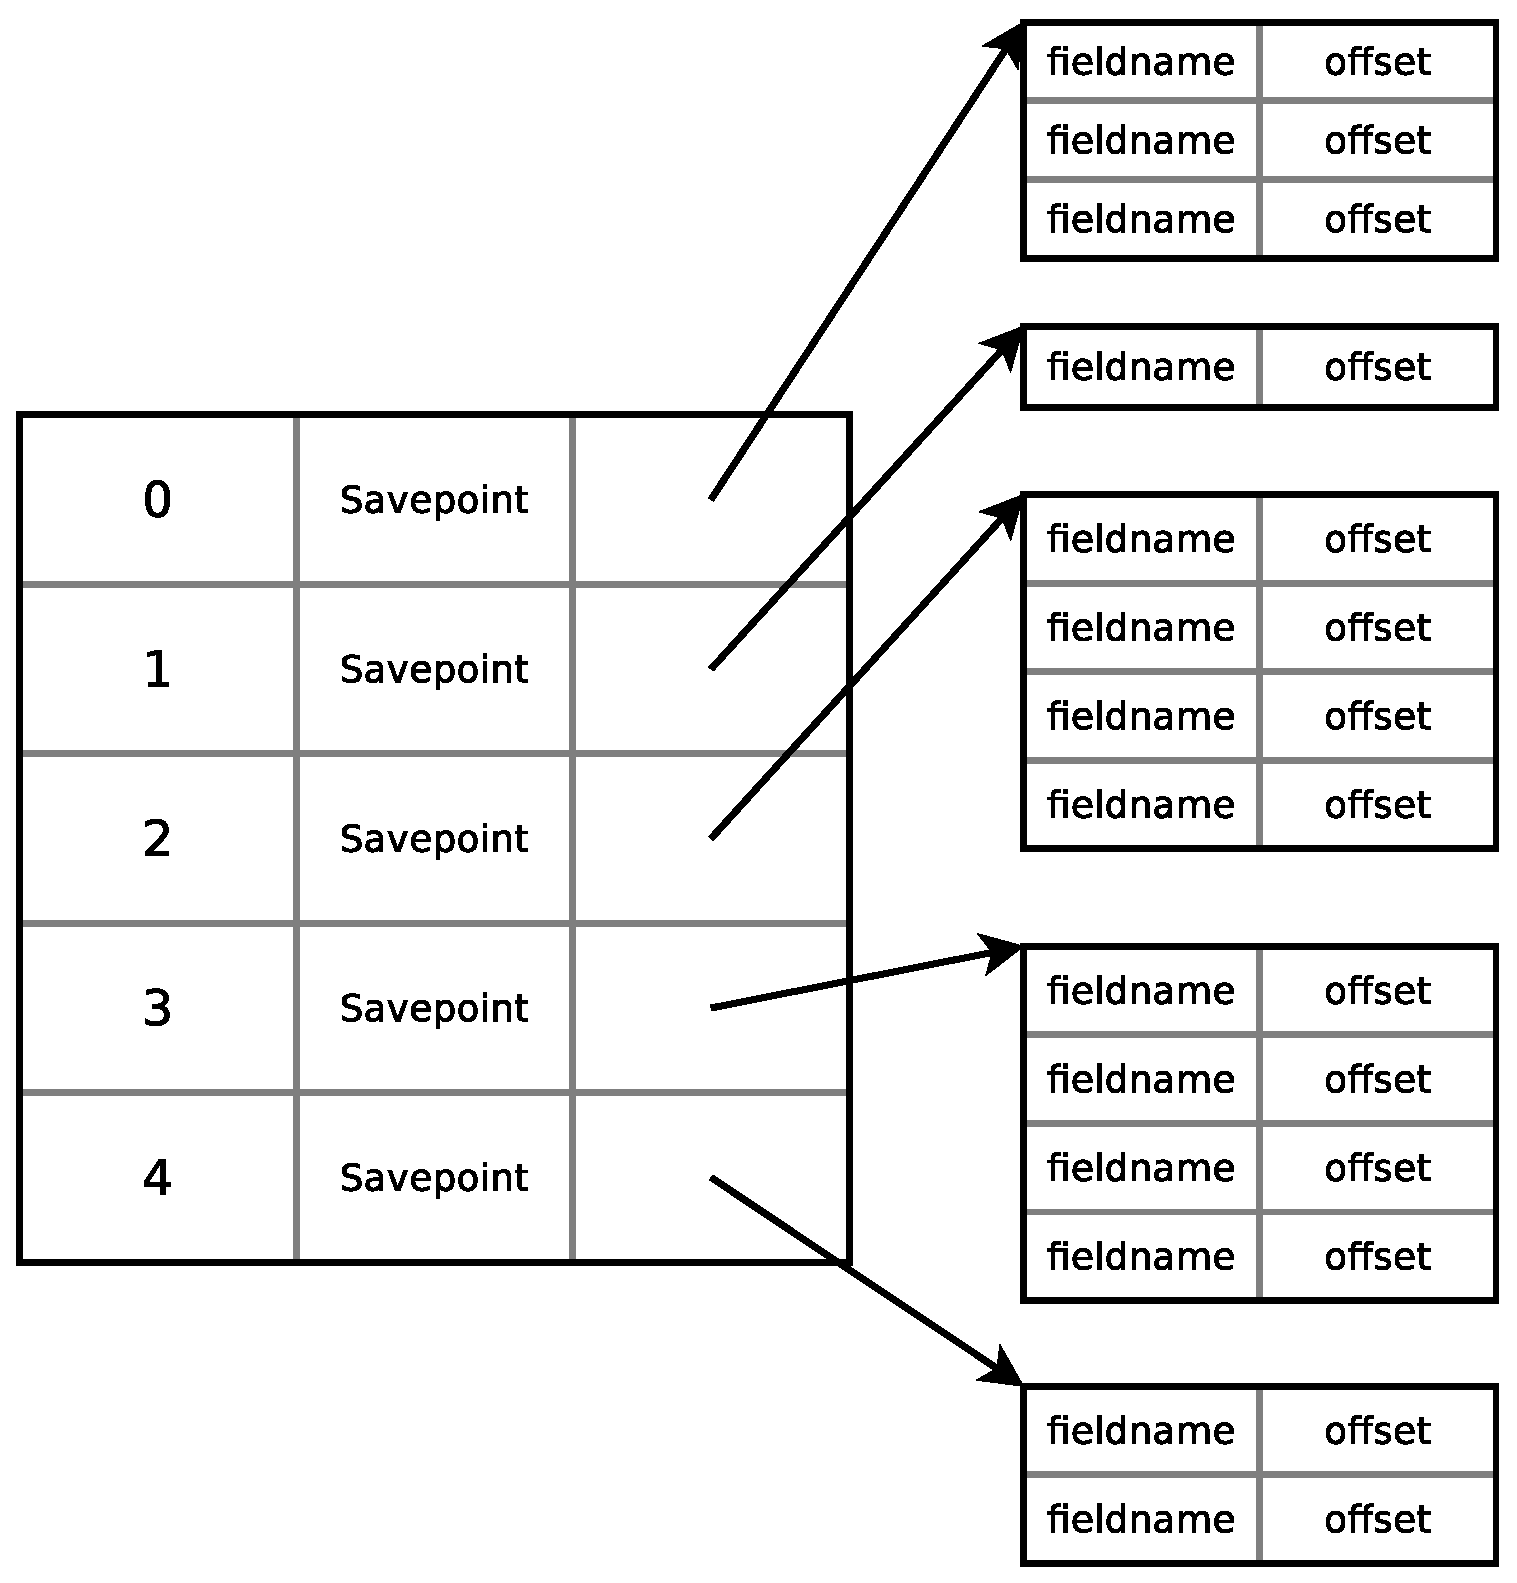
\includegraphics[width=0.85\textwidth]{./offsettable.eps}

 \caption{Offset table structure}
 \label{fig:offsettable}
\end{figure}

Finally, another structure not shown in the figure is the savepoint index: It 
is a map between the savepoints and their index in the vector of the savepoints
table.

Two operations are performed with the offset table: The write operation 
corresponds to adding a new triplet (fieldname, savepoint, offset), while 
the read operation corresponds to retrieving the offset given fieldname and 
savepoint.

To perform the write operation we need the index of the savepoint in the offset 
table. We can achieve this either by receiving it directly, or by doing a 
loopup in the savepoint index (which has a logarithmic cost in the number of 
savepoints). If the savepoint is not found in the index, a new row in the table 
and must by created: It will have an empty entry and its ID will be stored in 
the savepoint index. Once the ID of the entry in the table has been found, the 
map is searched for an occurrence of the fieldname: If such an occurrence 
exists, then we must raise an exception, since it is not allowed two have more 
than one instance of each field stored at one savepoint; otherwise, we update 
the map to contain the new entry \textit{fieldname} $\rightarrow$ 
\textit{offset}. As summary:

\begin{enumerate}
 \item Finding the savepoint ID (optional). Cost: $O(log(\#savepoints))$.
 \item Checking that entry does not contain \textit{fieldname} yet. \\
       Cost: $O\left(log(\#fields\ in\ savepoint)\right)$
 \item Adding the offset to the entry.
       Cost: $O\left(log(\#fields\ in\ savepoint)\right)$
\end{enumerate}

For the read operation we need the row ID as well. If the savepoint is not 
found in the savepoint index it we must throw an exception. Once the ID is 
known, we must access the entry to find the occurrence of the field. If the 
occurrence is not found, as exception must be thrown, otherwise the offset is 
returned. Summary:

\begin{enumerate}
 \item Finding the savepoint ID (optional). Cost: $O(log(\#savepoints))$.
 \item Accessing the entry to get the offset.
       Cost: $O\left(log(\#fields\ in\ savepoint)\right)$
\end{enumerate}

A final note: I was a bit inaccurate in the figure and in the explanation: the 
offset table entries to not only relate fieldnames to the respective offset, 
but to the respective pair offset/checksum: for each instance of the serialized 
fields we also have a checksum, which is used to avoid saving the same field 
content multiple times. The next section will explain more of it.

\section{Files and Directories}

A serializer represents a collection of fields serialized at determined
savepoints, as specified by the fields table and by the offset table.
How this collection is mirrored to the disk depends on the chosen file format.

The file format is an object implementing the interface specified by the pure 
virtual class \texttt{FileFormat}, and is responsible to decide where to write 
the organizational data and where to store binary data. The 
organizational data is a representation in JSON form of the tables described in 
Section \ref{datastructures}. Currently there is just one implementation 
of this interface: \texttt{CentralizedFileFormat}. With this format the 
organizational data is stored in a single file, while the binary data is stored 
separately for each field.

Whenever a field must be saved at a savepoint, the following operations are 
performed:

\begin{enumerate}
 \item The binary serializer creates a vector with serializer binary data and 
returns the checksum.
 \item The offset table checks if the field is already serialized in a previous 
savepoint with the same checksum.
 \item If there is a match, the offset is used; otherwise the serializer 
ask the file format where to put new binary data and takes the returned offset.
 \item The offset table is updated with the new offset.
\end{enumerate}

To read a field from file, the following operations are performed:

\begin{enumerate}
 \item The offset table returns the offset for the requested fieldname and 
savepoint.
 \item The serializer requests the file format to open the file in read mode at 
the returned offset.
 \item The binary data is read and passed to the binary serializer, which 
deserializes the data inside the multi-dimensional array in memory.
\end{enumerate}


\end{document}
